\documentclass[a4paper, 14pt]{extarticle}
\usepackage{enumitem}
\usepackage{fefutitle}
\usepackage{xcolor}
\usepackage{amsmath}
\usepackage{graphicx}
\usepackage[justification=centering]{caption}
\usepackage{float}

\begin{document}
	\fefutitle{3}
	\pagebreak	

	\section{Введение}
		В XIX веке рассматривались дифференциальные уравнения роста одновидовой популяции; они привели к моделям 		экспоненциального роста. Но для экологии одновидовая популяция — проблема слишком узкая, и особое значение придается работам А. Лотки и В. Вольтерра, в которых впервые появляются системы уравнений, относящиеся к многовидовым сообществам.
		
		Модель Лотки-Вольтерры является первоначальной и простейшей системой для описания модели «хищник-жертва», то есть популяции хищников и популяции жертв, взаимодействующих в какой-то среде: жертвы едят растительность, хищники — жертв
		
		В данной лабораторной будет реализована модель Лотки-Вольтерра - модель взаимодействия двух видов типа - <<хищник - жертва>>.
	\pagebreak
	\section{Создание математической модели}
		Рассматривается закрытый ареал, в котором обитают два вида: травоядные("жертва") и хищники. 
		\begin{figure}[H]
			\centering
			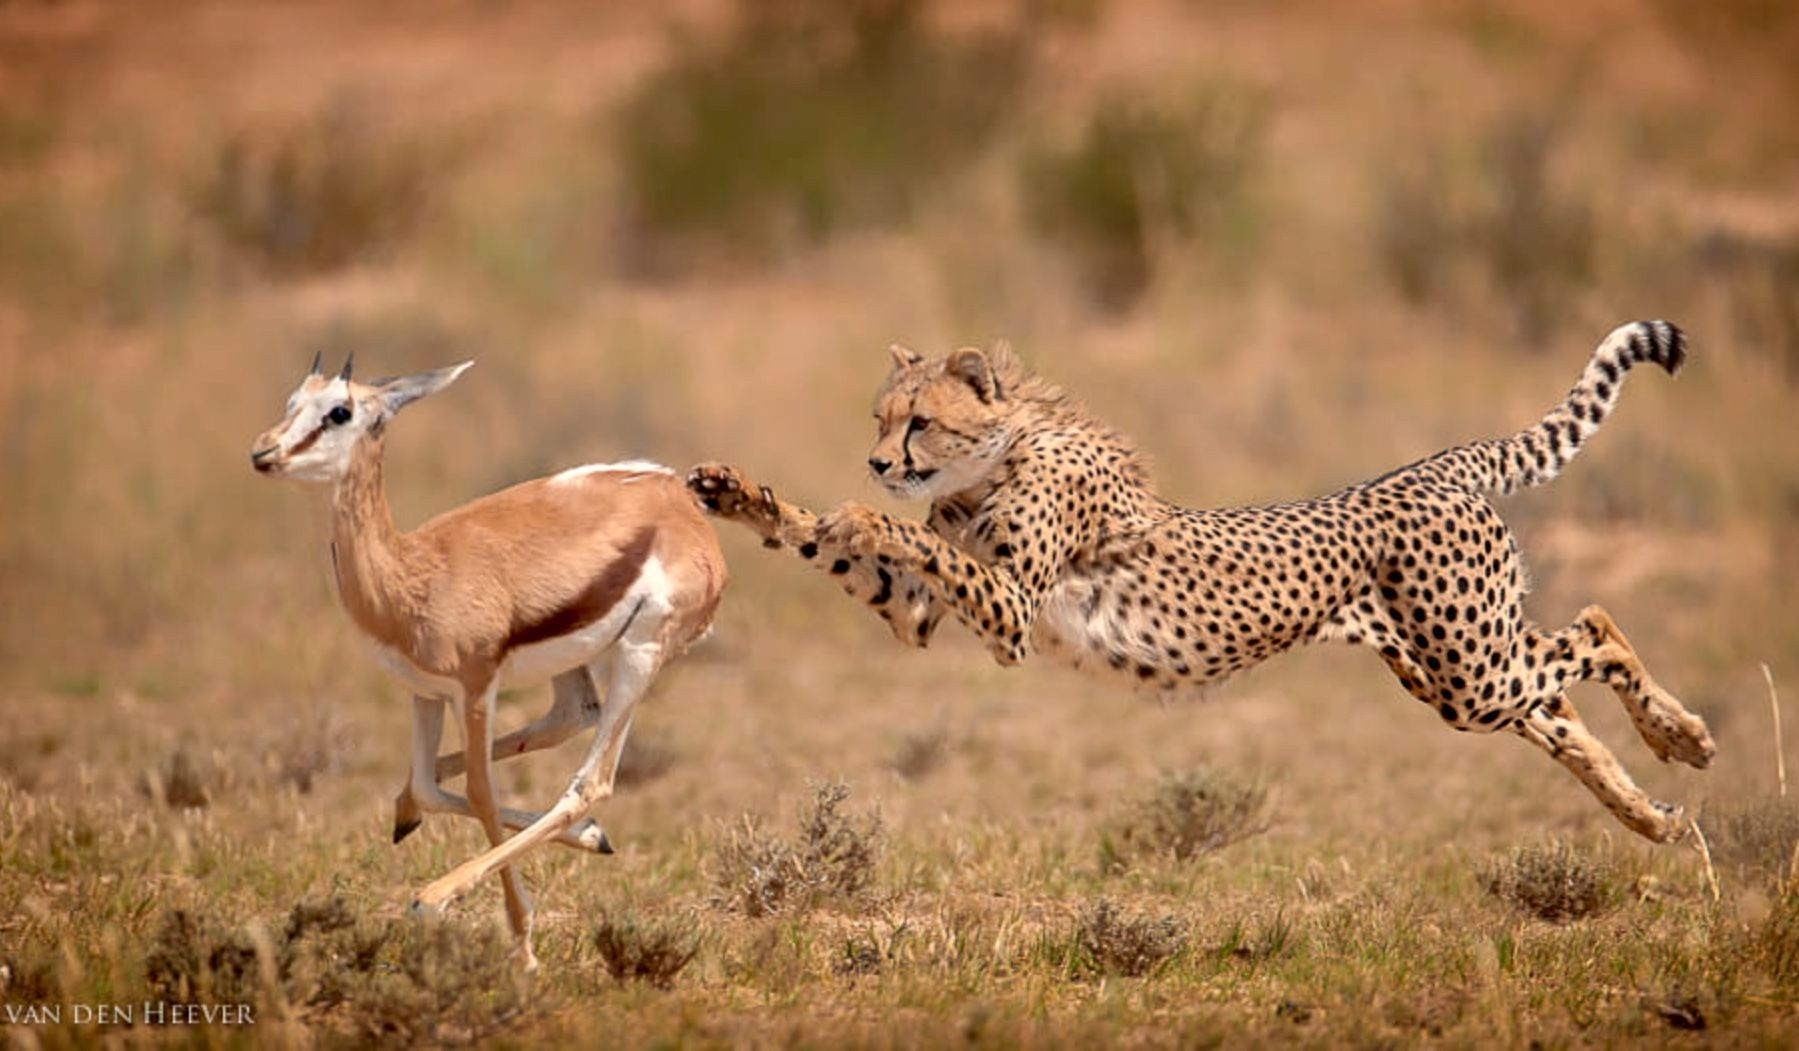
\includegraphics[width = \linewidth] {1.jpg}
			\caption[.] {Хищник и жертва}
		\end{figure}
		Предполагается, что животные не иммигрируют и не эмигрируют, и
		что еды для травоядных имеется с избытком. Тогда уравнение изменения количества жертв принимает вид:
			\[ \dfrac{dx}{dt} = \alpha x,\]
		где $\alpha$ - коэффициент рождаемости жертв, $x$ - величина популяции жертв, $\dfrac{dx}{dt}$ - скорость прироста популяции жертв

		Пока хищники не охотятся, они вымирают, следовательно, уравнение для численности хищников(без учета численности жертв) принимает вид:
			\[ \dfrac{dy}{dt} = -\gamma y,\]
		где $\gamma$ - коэффициент убыли хищников, $x$ - величина популяции хищников, $\dfrac{dx}{dt}$ - скорость прироста популяции хищников

		При встречах хищников и жертв(частота которых прямо пропорциональна величине $xy$) происходит убийство с коэффициентом $\beta$, сытые хищники способны к воспроизводству с коэффициентом $\delta$.
		С учетом этого, система уравнений модели такова:
		\[ \begin{cases}
			\dfrac{dx}{dt} = \alpha x - \beta xy = (\alpha - \beta y)x, \\
			\dfrac{dy}{dt} = - \gamma y + \delta xy = (\delta x - \gamma)y. \\
		    \end{cases}
		 \]
		 
	\section{Анализ модели}
		Найдём особые точки системы:
		\[ \begin{cases}
			(\alpha - \beta y)x = 0, \\
			(\delta x - \gamma)y = 0; \\
		\end{cases}
		\]
		
		\[ \begin{cases}
			\alpha x = \beta xy, \\
			\delta xy = \gamma; \\
		\end{cases}
		\]
		
		\[ \begin{cases}
			y(0) = \dfrac{\alpha}{\beta}, \\
			x(0) = \dfrac{\gamma}{\delta}; \\
		\end{cases}
		\]
	
	\pagebreak
	\section{Реализация модели}
		Модель была реализована в MathCad.
		\begin{figure}[H]
			\centering
			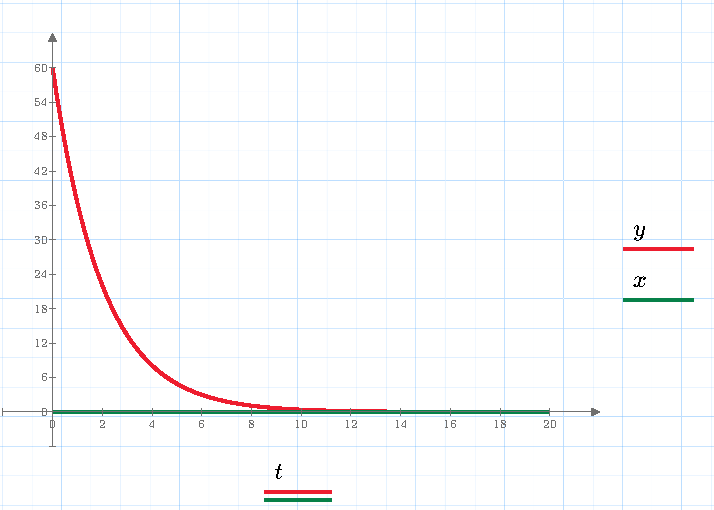
\includegraphics[width = \linewidth]{1.pdf}
			\caption[.] {}
		\end{figure}
		Если жертв(x) нет, то хищники(y) вымирают экспоненциально.
	
		\begin{figure}[H]
			\centering
			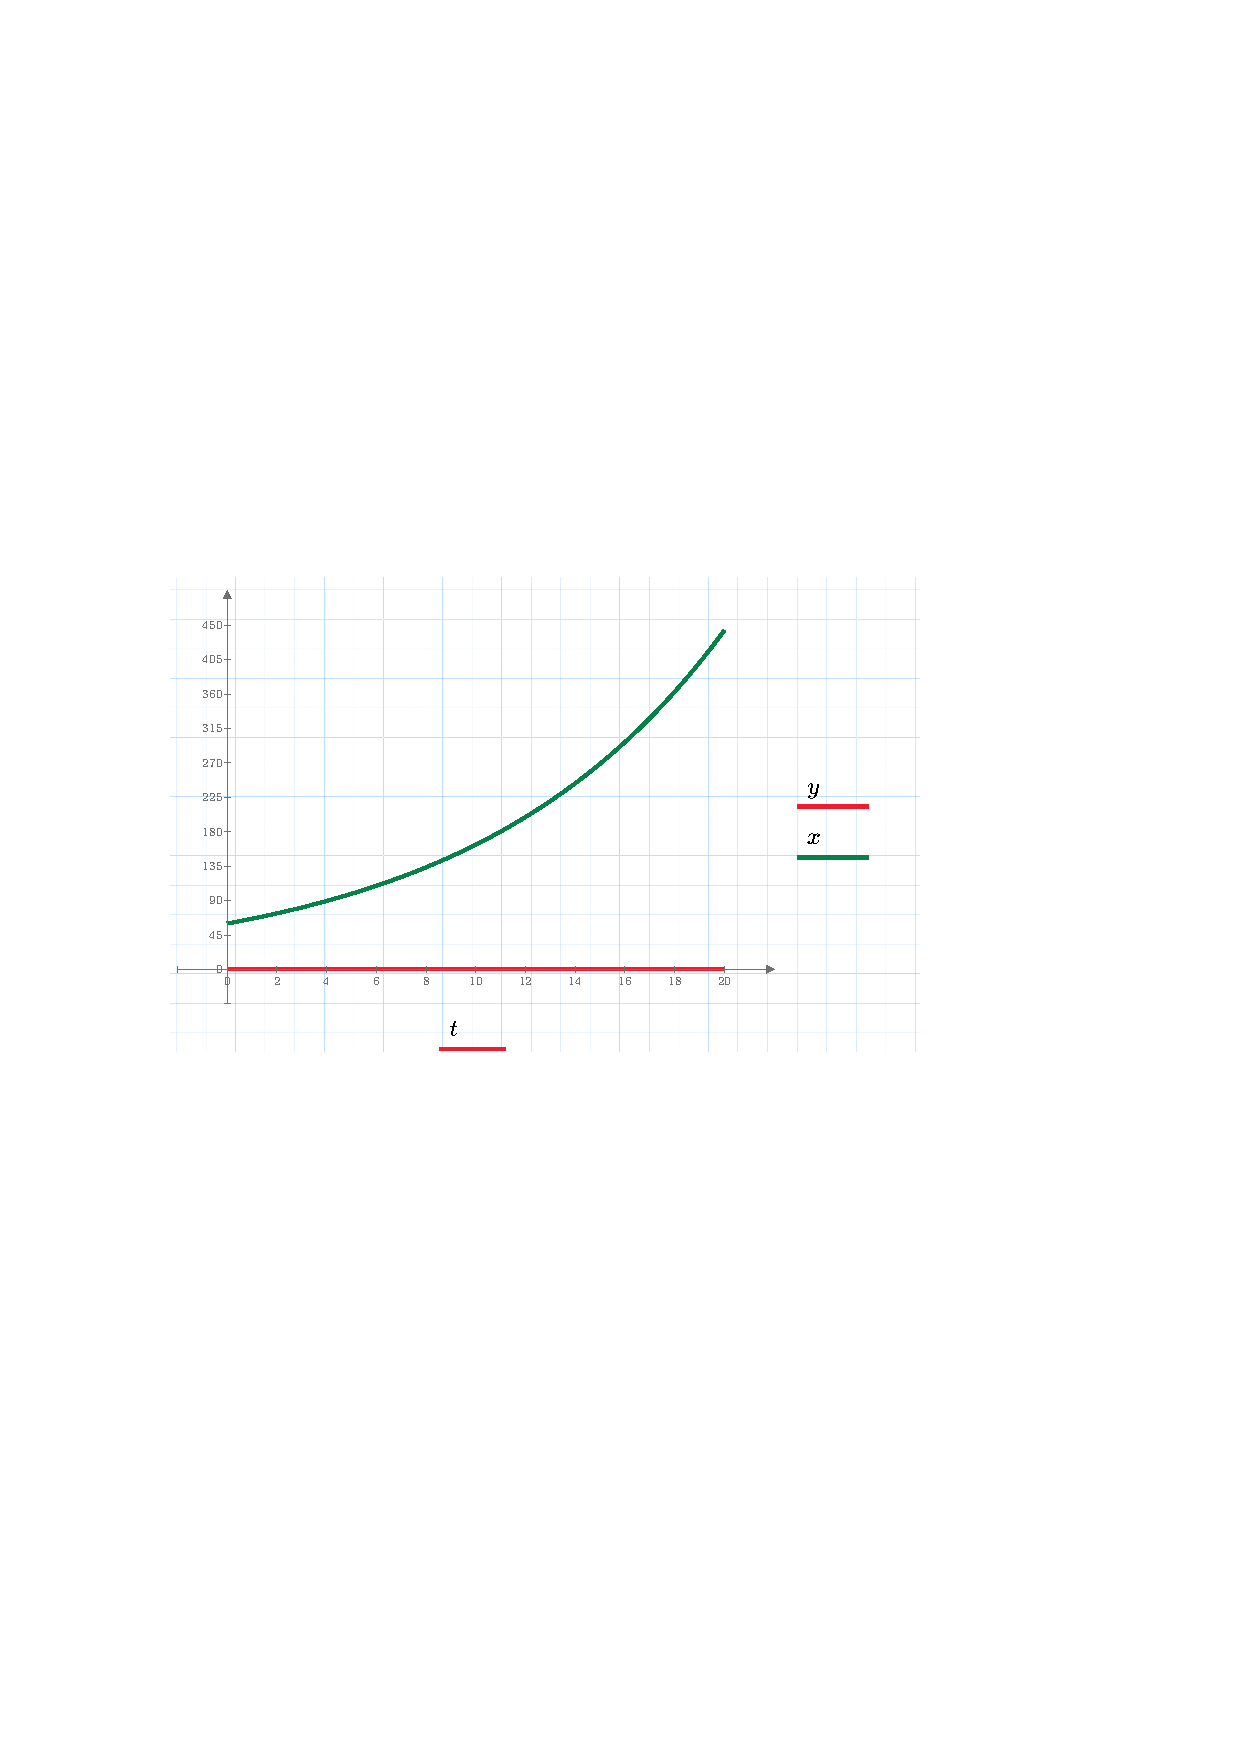
\includegraphics[width = \linewidth]{2.pdf}
			\caption[.] {}
		\end{figure}
		Если хищников(y) нет, то популяция жертв растет экспоненциально. 
		\pagebreak
		
		\noindent \[ x = \begin{bmatrix}
			4 \\ 5
		\end{bmatrix} \]
	
		\noindent\[
			\alpha = 2,\\
			\beta = 1,\\
			\gamma = 2,\\
			\delta = 1
		\]
		\begin{figure}[H]
			\centering
			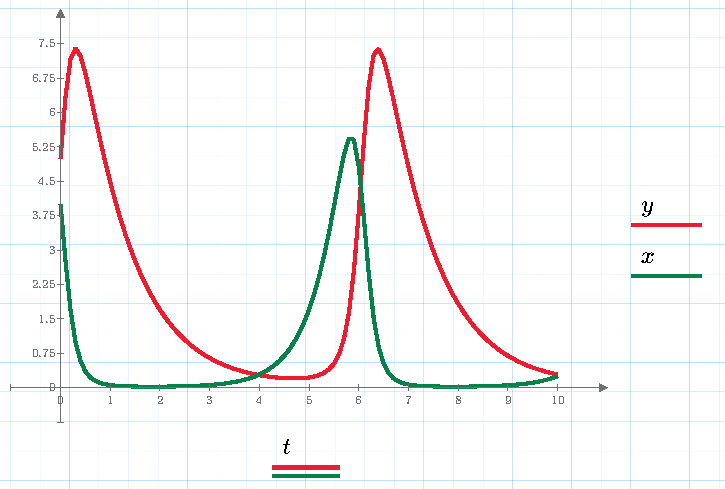
\includegraphics[width = \linewidth]{3.pdf}
			\caption[.] {}
		\end{figure}
		В начале периода количество жертв возрастает. Вместе с ними растет и количество хищников из-за обилия
		пищевых ресурсов. Активное поедание жертв приводит к снижению их количества. В следствии уменьшии пищи для хищников, они начинают вымирать. Цикл переодически повторяется.
		\pagebreak
		
		\noindent \[ x = \begin{bmatrix}
			4 \\ 5
		\end{bmatrix} \]
		
		\noindent\[
		\alpha = 2,\\
		\beta = 1,\\
		\gamma = 1,\\
		\delta = 1
		\]
		\begin{figure}[H]
			\centering
			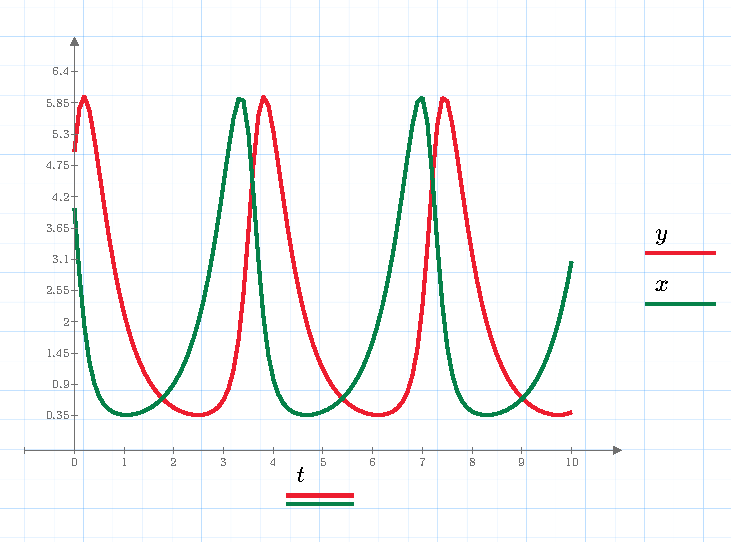
\includegraphics[width = \linewidth]{4.pdf}
			\caption[.] {}
		\end{figure}
		Увеличение естественной смертности хищников привело к тому, что период и максимальный размер популяции
		хищников уменьшились.
		\pagebreak
		
		\noindent \[ x = \begin{bmatrix}
			4 \\ 5
		\end{bmatrix} \]
		
		\noindent\[
		\alpha = 7,\\
		\beta = 1,\\
		\gamma = 1,\\
		\delta = 1
		\]
		\begin{figure}[H]
			\centering
			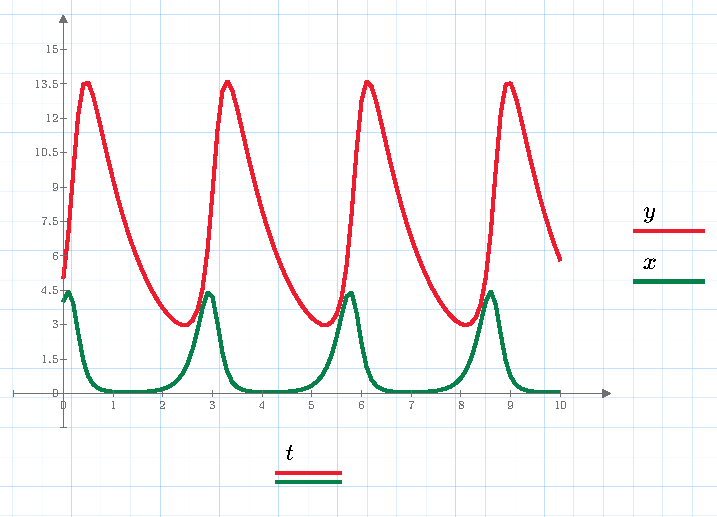
\includegraphics[width = \linewidth]{5.pdf}
			\caption[.] {}
		\end{figure}
		Увеличение рождаемости жертв приводит к уменьшению длительности периода и увеличению популяции хищников.
		\pagebreak
		
		\noindent \[ x = \begin{bmatrix}
			4 \\ 5
		\end{bmatrix} \]
		
		\noindent\[
		\alpha = 5,\\
		\beta = 1,\\
		\gamma = 4,\\
		\delta = 1
		\]
		\begin{figure}[H]
			\centering
			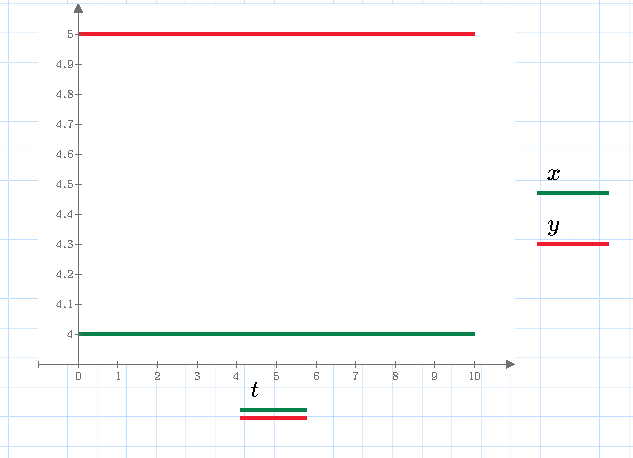
\includegraphics[width = \linewidth]{7.pdf}
			\caption[.] {}
		\end{figure}
		При данных параметрах система находится в равновесии: обе популяции неизменны и сбалансированы.
		\pagebreak
		
		Фазовый портрет при:
		\noindent \[
					x_0 = \begin{bmatrix} 4 \\ 4 \end{bmatrix}
					x_1 = \begin{bmatrix} 2 \\ 6 \end{bmatrix} 
					x_2 = \begin{bmatrix} 3 \\ 2 \end{bmatrix} 
					x_3 = \begin{bmatrix} 5 \\ 3 \end{bmatrix} 
					\]
		
		\noindent\[
		\alpha = 2,\\
		\beta = 0.5,\\
		\gamma = 1\\
		\delta = 0.5
		\]
		\begin{figure}[H]
			\centering
			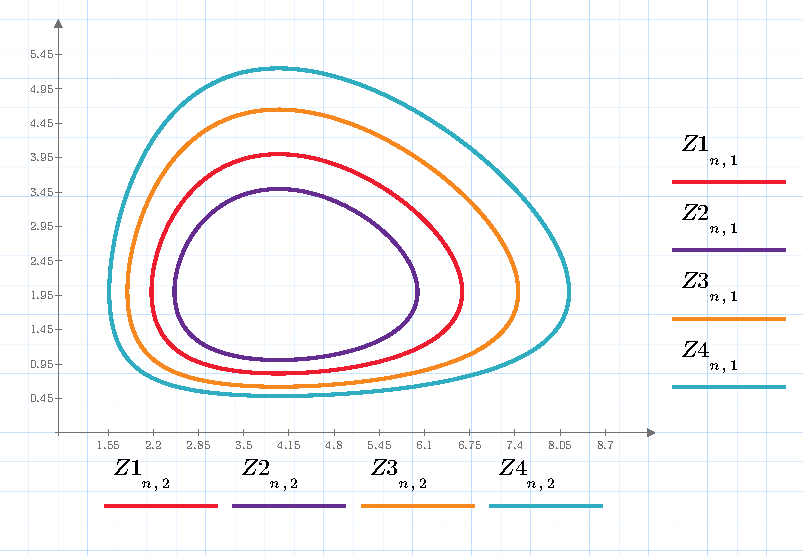
\includegraphics[width = \linewidth]{6.pdf}
			\caption[.] {}
		\end{figure}
	
	\section{Вывод}
		В ходе лабораторной работы была изучена модель Лотки-Вольтерры и реализована с помощью программы
		Mathcad при разных параметрах. 
		
\end{document}	